\chapter{UNet Test Model Implementation with MONAI}
\label{ch:unet_model}
To gain a better understanding of the data and task at hand, we first implement a simple UNet model using the MONAI framework. This serves as a baseline implementation before developing our own custom model architecture in later stages.

\section{MONAI Pipeline Overview}
\label{sec:monai_pipeline}

% Content to be added about the MONAI pipeline implementation

\section{UNet Architecture}
\label{sec:unet_architecture}

% Content to be added about the specific UNet architecture used

\section{Implementation}
\label{sec:implementation}

The Python libraries MONAI and PyTorch offer a wealth of features that facilitate the implementation of a UNet model. One useful feature is \texttt{monai.transforms}, which provides a range of transformations for data preprocessing.

To train a UNet model on volumetric data using MONAI, it is essential that all inputs in a batch share the same spatial dimensions. If the spatial dimensions differ, stacking the data into a 5D tensor will fail. Additionally, the image and its corresponding mask must be congruent in shape and distance. Therefore, a preprocessing pipeline is required to:

\begin{enumerate}
    \item Unify spacings by resampling to a uniform voxel spacing
    \item Center and crop the data to a common region of interest (ROI)
    \item Apply padding to ensure a fixed size
\end{enumerate}

Furthermore, it is necessary to apply these transformations synchronously to both the image and the mask.

For example:

\begin{itemize}
    \item Voxel spacing is unified using the transformation \texttt{Spacingd(keys=["image", "label"], pixdim=[1.0, 1.0, 1.0])}, ensuring that all voxels have the same spacing along each axis (the physical distance between the centers of adjacent voxels)
    \item The voxel shape must be divisible by a factor $k$, which is enforced by \texttt{DivisiblePadd(keys=["image", "label"], k=16)}
  
\end{itemize}

We begin by implementing a minimal viable model that uses the Binary Cross-Entropy (BCE) loss function and the Dice metric. The model is trained on a single batch for five epochs, taking approximately 10 minutes. The results after training are:

\begin{itemize}
    \item Loss: 0.1655
    \item Dice: 0.0000
\end{itemize}

\begin{figure}[htbp]
    \centering
    \begin{subfigure}{\textwidth}
        \centering
        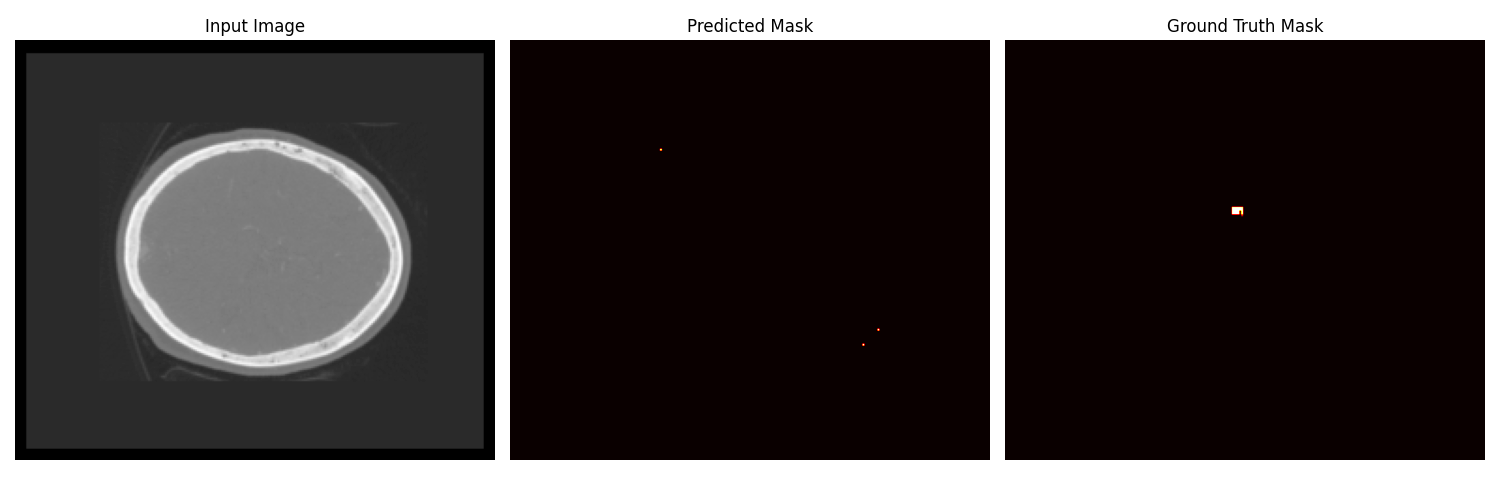
\includegraphics[width=\textwidth]{figures/Figure_2.png}
        \caption{Axiale Ansicht eines CT-Scans mit zugehöriger Vorhersage und Ground Truth Maske. Die Vorhersage zeigt keine Übereinstimmung mit der tatsächlichen Läsion.}
        \label{fig:predicted_mask_axial}
    \end{subfigure}
    \vspace{1em}
    \begin{subfigure}{\textwidth}
        \centering
        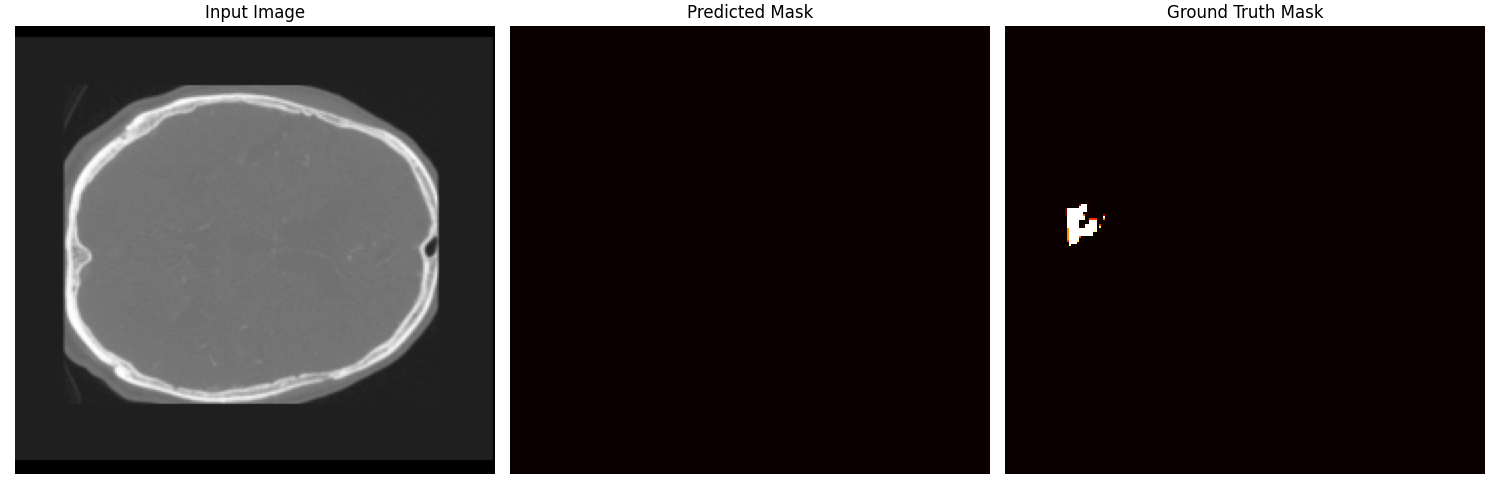
\includegraphics[width=\textwidth]{figures/Figure_3.png}
        \caption{Koronale Ansicht desselben CT-Scans. Auch hier ist deutlich zu erkennen, dass das Modell die Läsion nicht korrekt segmentiert.}
        \label{fig:predicted_mask_coronal}
    \end{subfigure}
    \caption{Vergleich zwischen Input-Bild (links), vorhergesagter Maske (Mitte) und Ground Truth Maske (rechts) für zwei verschiedene Schnittebenen. Die schwarzen Vorhersagemasken zeigen, dass das Modell hauptsächlich den Hintergrund vorhersagt und die Läsionen nicht erkennt.}
    \label{fig:prediction_comparison}
\end{figure}

A Dice score of 0 implies that the model is not matching the target masks at all, which likely means the model is either not detecting any relevant features or making entirely incorrect predictions. To further investigate, we visualize both the predicted mask and the ground truth mask. As shown in Figure~\ref{fig:prediction_comparison}, the predicted mask does not resemble the ground truth, despite the loss being relatively low. The model seems to be predicting only the background, failing to capture the lesion area.

Upon further analysis, we found that the BCE loss function is not well-suited for this problem. This is due to the fact that the positive class (the lesion) is often much smaller than the background. Using BCE encourages the model to focus on the background, leading to:

\begin{itemize}
    \item False negatives, where small lesions are barely penalized
    \item Uneven learning, where the model learns to detect background features rather than the lesion itself
\end{itemize}

In contrast, the Dice loss function is more appropriate for this task, as it directly maximizes the spatial overlap between the predicted mask and the ground truth, which is crucial when dealing with imbalanced datasets like this.

\section{Dice Loss Function}
\label{sec:dice_loss}

The Dice loss function is commonly used in medical image segmentation tasks due to its effectiveness in handling class imbalance, which is typical in medical imaging where the region of interest (e.g., lesions) often occupies only a small portion of the image.

\begin{figure}[htbp]
    \centering
    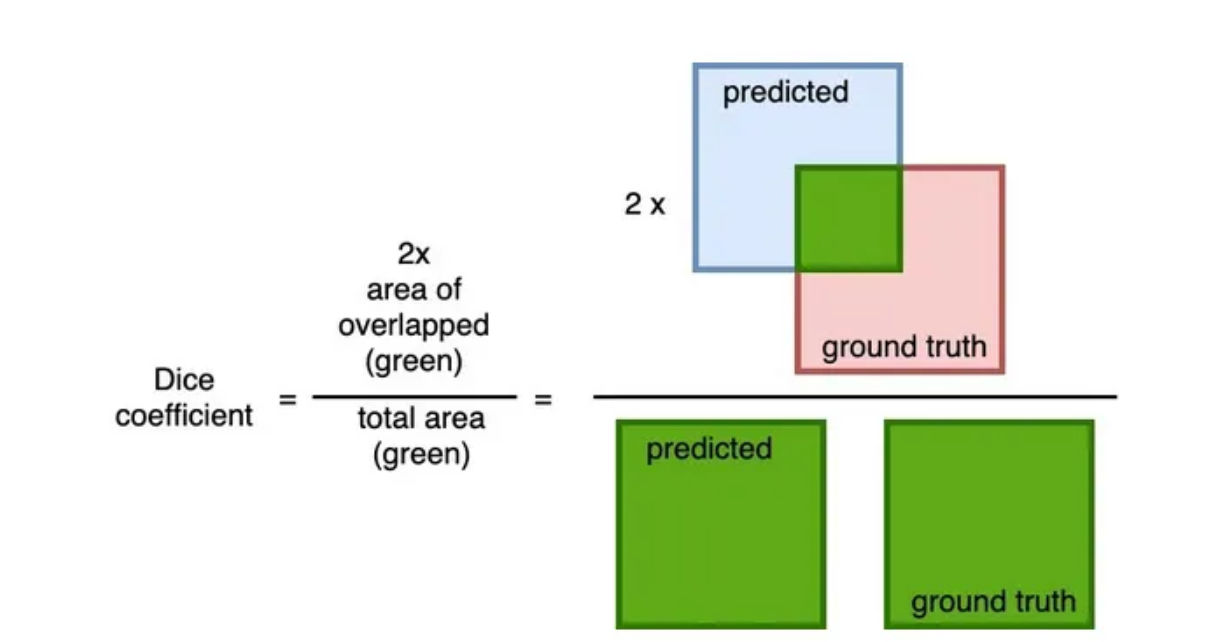
\includegraphics[width=0.7\textwidth]{figures/dice_loss_illustration.png}
    \caption{Visual explanation of the Dice coefficient calculation. The Dice coefficient is computed as the ratio of twice the area of overlap (green) to the total area of both the predicted segmentation and ground truth. Image adapted from \cite{nevilledice2023}.}
    \label{fig:dice_illustration}
\end{figure}

The Dice loss is derived from the Dice coefficient (also known as F1 score), which measures the overlap between the predicted segmentation and the ground truth. The Dice coefficient is defined as:

\begin{equation}
\text{Dice} = \frac{2 |X \cap Y|}{|X| + |Y|}
\end{equation}

where $X$ is the predicted set and $Y$ is the ground truth set. 

